
\documentclass[letterpaper,hide notes,xcolor={table,svgnames},pdftex]{beamer}
\def\showexamples{t}


%\usepackage[svgnames]{xcolor}

%% Demo talk
%\documentclass[letterpaper,notes=show]{beamer}

\usecolortheme{crane}%seahorse crane
\setbeamertemplate{navigation symbols}{}

\usetheme{MyPittsburgh}
%\usetheme{Frankfurt}

%\usepackage{tipa}

\usepackage{hyperref}
\usepackage{graphicx,xspace}
\usepackage[normalem]{ulem}

\newcommand\SF[1]{$\bigstar$\footnote{SF: #1}}

\usepackage{paratype}
\renewcommand*\familydefault{\sfdefault} %% Only if the base font of the document is to be sans serif
\usepackage[zerostyle=c]{newtxtt}
\usepackage[T1]{fontenc}

\newcounter{tmpnumSlide}
\newcounter{tmpnumNote}

\usepackage{xcolor}
\usepackage{tabu}
\definecolor{light-gray}{gray}{0.75}
\taburulecolor{light-gray}

% old question code
%\newcommand\question[1]{{$\bigstar$ \small \onlySlide{2}{#1}}}
% \newcommand\nquestion[1]{\ifdefined \presentationonly \textcircled{?} \fi \note{\par{\Large \textbf{?}} #1}}
% \newcommand\nanswer[1]{\note{\par{\Large \textbf{A}} #1}}


 \newcommand\mnote[1]{%
   \addtocounter{tmpnumSlide}{1}
   \ifdefined\showcues {~\tiny\fbox{\arabic{tmpnumSlide}}}\fi
   \note{\setlength{\parskip}{1ex}\addtocounter{tmpnumNote}{1}\textbf{\Large \arabic{tmpnumNote}:} {#1\par}}}

\newcommand\mmnote[1]{\note{\setlength{\parskip}{1ex}#1\par}}

%\newcommand\mnote[2][]{\ifdefined\handoutwithnotes {~\tiny\fbox{#1}}\fi
% \note{\setlength{\parskip}{1ex}\textbf{\Large #1:} #2\par}}

%\newcommand\mnote[2][]{{\tiny\fbox{#1}} \note{\setlength{\parskip}{1ex}\textbf{\Large #1:} #2\par}}

\newcommand\mquestion[2]{{~\color{red}\fbox{?}}\note{\setlength{\parskip}{1ex}\par{\Large \textbf{?}} #1} \note{\setlength{\parskip}{1ex}\par{\Large \textbf{A}} #2\par}\ifdefined \presentationonly \pause \fi}

\newcommand\blackboard[1]{%
\ifdefined   \showblackboard
  {#1}
  \else {\begin{center} \fbox{\colorbox{blue!30}{%
         \begin{minipage}{.95\linewidth}%
           \hspace{\stretch{1}} Some space intentionally left blank; done at the blackboard.%
         \end{minipage}}}\end{center}}%
         \fi%
}



%\newcommand\q{\tikz \node[thick,color=black,shape=circle]{?};}
%\newcommand\q{\ifdefined \presentationonly \textcircled{?} \fi}

\usepackage{listings}
\lstset{%
  keywordstyle=\bfseries,
  aboveskip=15pt,
  belowskip=15pt,
  captionpos=b,
  identifierstyle=\ttfamily,
  escapeinside={(*@}{@*)},
  stringstyle=\ttfamiliy,
  frame=lines,
  numbers=left, basicstyle=\scriptsize, numberstyle=\tiny, stepnumber=0, numbersep=2pt}

\usepackage{siunitx}
\newcommand\sius[1]{\num[group-separator = {,}]{#1}\si{\micro\second}}
\newcommand\sims[1]{\num[group-separator = {,}]{#1}\si{\milli\second}}
\newcommand\sins[1]{\num[group-separator = {,}]{#1}\si{\nano\second}}
\sisetup{group-separator = {,}, group-digits = true}

%% -------------------- tikz --------------------
\usepackage{tikz}
\usetikzlibrary{positioning}
\usetikzlibrary{arrows,backgrounds,automata,decorations.shapes,decorations.pathmorphing,decorations.markings,decorations.text}

\tikzstyle{place}=[circle,draw=blue!50,fill=blue!20,thick, inner sep=0pt,minimum size=6mm]
\tikzstyle{transition}=[rectangle,draw=black!50,fill=black!20,thick, inner sep=0pt,minimum size=4mm]

\tikzstyle{block}=[rectangle,draw=black, thick, inner sep=5pt]
\tikzstyle{bullet}=[circle,draw=black, fill=black, thin, inner sep=2pt]

\tikzstyle{pre}=[<-,shorten <=1pt,>=stealth',semithick]
\tikzstyle{post}=[->,shorten >=1pt,>=stealth',semithick]
\tikzstyle{bi}=[<->,shorten >=1pt,shorten <=1pt, >=stealth',semithick]

\tikzstyle{mut}=[-,>=stealth',semithick]

\tikzstyle{treereset}=[dashed,->, shorten >=1pt,>=stealth',thin]

\usepackage{ifmtarg}
\usepackage{xifthen}
\makeatletter
% new counter to now which frame it is within the sequence
\newcounter{multiframecounter}
% initialize buffer for previously used frame title
\gdef\lastframetitle{\textit{undefined}}
% new environment for a multi-frame
\newenvironment{multiframe}[1][]{%
\ifthenelse{\isempty{#1}}{%
% if no frame title was set via optional parameter,
% only increase sequence counter by 1
\addtocounter{multiframecounter}{1}%
}{%
% new frame title has been provided, thus
% reset sequence counter to 1 and buffer frame title for later use
\setcounter{multiframecounter}{1}%
\gdef\lastframetitle{#1}%
}%
% start conventional frame environment and
% automatically set frame title followed by sequence counter
\begin{frame}%
\frametitle{\lastframetitle~{\normalfont(\arabic{multiframecounter})}}%
}{%
\end{frame}%
}
\makeatother

\makeatletter
\newdimen\tu@tmpa%
\newdimen\ydiffl%
\newdimen\xdiffl%
\newcommand\ydiff[2]{%
    \coordinate (tmpnamea) at (#1);%
    \coordinate (tmpnameb) at (#2);%
    \pgfextracty{\tu@tmpa}{\pgfpointanchor{tmpnamea}{center}}%
    \pgfextracty{\ydiffl}{\pgfpointanchor{tmpnameb}{center}}%
    \advance\ydiffl by -\tu@tmpa%
}
\newcommand\xdiff[2]{%
    \coordinate (tmpnamea) at (#1);%
    \coordinate (tmpnameb) at (#2);%
    \pgfextractx{\tu@tmpa}{\pgfpointanchor{tmpnamea}{center}}%
    \pgfextractx{\xdiffl}{\pgfpointanchor{tmpnameb}{center}}%
    \advance\xdiffl by -\tu@tmpa%
}
\makeatother
\newcommand{\copyrightbox}[3][r]{%
\begin{tikzpicture}%
\node[inner sep=0pt,minimum size=2em](ciimage){#2};
\usefont{OT1}{phv}{n}{n}\fontsize{4}{4}\selectfont
\ydiff{ciimage.south}{ciimage.north}
\xdiff{ciimage.west}{ciimage.east}
\ifthenelse{\equal{#1}{r}}{%
\node[inner sep=0pt,right=1ex of ciimage.south east,anchor=north west,rotate=90]%
{\raggedleft\color{black!50}\parbox{\the\ydiffl}{\raggedright{}#3}};%
}{%
\ifthenelse{\equal{#1}{l}}{%
\node[inner sep=0pt,right=1ex of ciimage.south west,anchor=south west,rotate=90]%
{\raggedleft\color{black!50}\parbox{\the\ydiffl}{\raggedright{}#3}};%
}{%
\node[inner sep=0pt,below=1ex of ciimage.south west,anchor=north west]%
{\raggedleft\color{black!50}\parbox{\the\xdiffl}{\raggedright{}#3}};%
}
}
\end{tikzpicture}
}


%% --------------------

%\usepackage[excludeor]{everyhook}
%\PushPreHook{par}{\setbox0=\lastbox\llap{MUH}}\box0}

%\vspace*{\stretch{1}

%\setbox0=\lastbox \llap{\textbullet\enskip}\box0}

\setlength{\parskip}{\fill}

\newcommand\noskips{\setlength{\parskip}{1ex}}
\newcommand\doskips{\setlength{\parskip}{\fill}}

\newcommand\xx{\par\vspace*{\stretch{1}}\par}
\newcommand\xxs{\par\vspace*{2ex}\par}
\newcommand\tuple[1]{\langle #1 \rangle}
\newcommand\code[1]{{\sf \footnotesize #1}}
\newcommand\ex[1]{\uline{Example:} \ifdefined \presentationonly \pause \fi
  \ifdefined\showexamples#1\xspace\else{\uline{\hspace*{2cm}}}\fi}

\newcommand\ceil[1]{\lceil #1 \rceil}


\AtBeginSection[]
{
   \begin{frame}
       \frametitle{Outline}
       \tableofcontents[currentsection]
   \end{frame}
}



\pgfdeclarelayer{edgelayer}
\pgfdeclarelayer{nodelayer}
\pgfsetlayers{edgelayer,nodelayer,main}

\tikzstyle{none}=[inner sep=0pt]
\tikzstyle{rn}=[circle,fill=Red,draw=Black,line width=0.8 pt]
\tikzstyle{gn}=[circle,fill=Lime,draw=Black,line width=0.8 pt]
\tikzstyle{yn}=[circle,fill=Yellow,draw=Black,line width=0.8 pt]
\tikzstyle{empty}=[circle,fill=White,draw=Black]
\tikzstyle{bw} = [rectangle, draw, fill=blue!20, 
    text width=4em, text centered, rounded corners, minimum height=2em]
    
    \newcommand{\CcNote}[1]{% longname
	This work is licensed under the \textit{Creative Commons #1 3.0 License}.%
}
\newcommand{\CcImageBy}[1]{%
	\includegraphics[scale=#1]{creative_commons/cc_by_30.pdf}%
}
\newcommand{\CcImageSa}[1]{%
	\includegraphics[scale=#1]{creative_commons/cc_sa_30.pdf}%
}
\newcommand{\CcImageNc}[1]{%
	\includegraphics[scale=#1]{creative_commons/cc_nc_30.pdf}%
}
\newcommand{\CcGroupBySa}[2]{% zoom, gap
	\CcImageBy{#1}\hspace*{#2}\CcImageNc{#1}\hspace*{#2}\CcImageSa{#1}%
}
\newcommand{\CcLongnameByNcSa}{Attribution-NonCommercial-ShareAlike}


\newenvironment{changemargin}[1]{% 
  \begin{list}{}{% 
    \setlength{\topsep}{0pt}% 
    \setlength{\leftmargin}{#1}% 
    \setlength{\rightmargin}{1em}
    \setlength{\listparindent}{\parindent}% 
    \setlength{\itemindent}{\parindent}% 
    \setlength{\parsep}{\parskip}% 
  }% 
  \item[]}{\end{list}} 




\title{Lecture 23 --- Library Functions }

\author{J. Zarnett\\
\texttt{jzarnett@uwaterloo.ca}}
\institute{Department of Electrical and Computer Engineering \\
  University of Waterloo}
\date{\today}

\begin{document}

\begin{frame}
  \titlepage
  
  \begin{center}
  \small{Acknowledgments: W.D. Bishop}
  \end{center}
\end{frame}


\begin{frame}
\frametitle{Library Functions}
The system provides a number of classes and types (in various namespaces, like \texttt{System.Console}) for programmers' use.

We often ask students, as exercises, to implement functions like absolute value or exponentiation.

In practical situations, these functions are already available to us as static methods of specific classes.

Many of the built-in classes are in the \texttt{System} namespace.\\
\quad Or in a namespace enclosed within \texttt{System}, like \texttt{System.Console}.

\end{frame}

\begin{frame}
\frametitle{\texttt{Math} Class}
Example: the \texttt{System.Math} class contains a number of different mathematical operations, including, but not limited to:

\begin{center}
\begin{tabular}{l l}
\textbf{Function} & \textbf{Returns}\\ \hline
\texttt{Abs} & Absolute Value\\
\texttt{Cos} & Cosine\\
\texttt{Max} & The larger of two values\\
\texttt{Round} & The closest integer\\
\end{tabular}
\end{center}

The usage is straightforward:\\
\quad \texttt{double z = Math.Pow( x, y );}

The object is \texttt{Math}, and \texttt{Pow} is a static method. \\
\quad There is no specific instance of \texttt{Math} created.

\end{frame}

\begin{frame}[fragile]
\frametitle{Example: Using the \texttt{Math} Class}

The following code:

\begin{verbatim}
double d = -3.14;
Console.WriteLine( Math.Abs( d ) );
Console.WriteLine( Math.Floor( d ) );
Console.WriteLine( Math.Round( Math.Abs( d ) ) );
\end{verbatim}

... produces as output:\\
\texttt{3.14\\
-4\\
3}

\end{frame}


\begin{frame}
\frametitle{Static Classes}
In fact, an instantiation like \texttt{new Math()} makes no sense.\\
\quad The class \texttt{Math} is declared as \texttt{static}.\\
\quad Therefore such an instantiation cannot take place.

A \texttt{static} class may not be instantiated; there is only one copy of it.\\
\quad Accordingly, no instance constructor may be created.

As you would expect, a static class may contain only static members (variables as well as methods).

\end{frame}

\begin{frame}
\frametitle{Static Classes}

Creating a static class is therefore basically the same as creating a class that contains only static members and a private constructor. 

Recall: a private method cannot be called from outside the class.

A private constructor prevents instantiation from outside the class. If the class contains no such instantiation, it will never be instantiated.

The advantage of using a static class is that the compiler can check to make sure that no instance members are accidentally added. 

The compiler ensures that instances of this class cannot be created.

\end{frame}



\begin{frame}
\frametitle{Examining Value Types}

It's not only the system-provided namespaces and classes that have functions available to use; even built-in types have some!

You may have wondered how a built-in value type can parse input.

In reality, the C\# built-in value types are aliases for structured types.

For example, the \texttt{int} type is really a \texttt{struct} that defines:
\begin{itemize}
	\item Constants for MinValue and MaxValue
	\item Methods for parsing, string conversion, comparison, and other operations common to all value types 
\end{itemize}

\end{frame}

\begin{frame}
\frametitle{Simple Types}
Simple types can be represented by the following diagram:

\begin{center}
	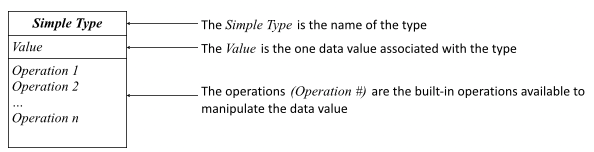
\includegraphics[width=\textwidth]{images/simpletype.png}
\end{center}

Different types will have different methods associated with them.

\end{frame}



\begin{frame}
\frametitle{The \texttt{char} Type Static Methods}
The \texttt{char} type defines a built-in type, but in C\# it's also a \texttt{struct} called \texttt{System.char} that provides static methods to test characters:

\begin{center}
\begin{tabular}{l|l}
	\textbf{Static Method} & \textbf{Checks if }\texttt{ch}\textbf{ is ...} \\ \hline
	
\texttt{IsDigit( char ch )} &  A digit\\ \hline
\texttt{IsLetter( char ch )} &  A letter\\ \hline
\texttt{IsLetterOrDigit( char ch )} &  A letter or a digit\\ \hline
\texttt{IsLower( char ch )} &  A lowercase letter\\ \hline
\texttt{IsUpper( char ch )} &  An uppercase letter\\ \hline
\texttt{IsWhiteSpace( char ch )} &  A white space character\\ 
	
\end{tabular}
\end{center}

(Don't attempt to memorize this table.)
\end{frame}

\begin{frame}
\frametitle{Using \texttt{char} Type Static Methods}

When reading data in from the user with \texttt{Console.ReadLine()}, we have sometimes parsed it into a number type.

This has resulted in an Exception if the user entered some letters or other garbage data where a number was expected.

Though we now know how to handle an Exception with the try-catch statement, we can now check the input before parsing.

Because strings are just arrays of characters, we can use the \texttt{char} static methods on individual characters within a string.

\end{frame}

\begin{frame}[fragile]
\frametitle{Using \texttt{char} Type Static Methods}

\begin{verbatim}
String input = Console.ReadLine( );
bool validInput = false;
while( !validInput )
{
    for ( char c in input )
    {
        if( !char.isDigit( c ) )
        {
            break;
        }
    }
    validInput = true;
}
int parsedValue = int.Parse( input );
\end{verbatim}

But what if the input is empty...?

\end{frame}


\begin{frame}
\frametitle{The \texttt{string} Type Search Methods}
The \texttt{string} type provides many methods to help you work with them:

{\scriptsize
\begin{center}
\begin{tabular}{l|p{5cm}}
	\textbf{Method} & \textbf{Returns} \\ \hline
	
\texttt{bool s1.StartsWith( string s2 )} & true if \texttt{s1} begins exactly with \texttt{s2}\\ \hline
\texttt{bool s1.EndsWith( string s2 )} & true if \texttt{s1} ends exactly with \texttt{s2}\\ \hline
\texttt{int s1.IndexOf( char ch )} & the first position of \texttt{ch} within \texttt{s1}\\ \hline
\texttt{int s1.IndexOf( char ch, int pos )} & the first position of \texttt{ch} within \texttt{s1} after (pos~-~1)\\ \hline
\texttt{int s1.IndexOf( string s2 )} & the first position of \texttt{s2} within \texttt{s1}\\ \hline
\texttt{int s1.IndexOf( string s2, int pos )} & the first position of \texttt{s2} within \texttt{s1} after (pos~-~1)\\ \hline
\texttt{string s1.Substring( int pos )} & a copy of the substring from \texttt{s1} starting at index pos and ending at the end of \texttt{s1}\\ \hline
\texttt{string s1.Substring( int pos, int len )} & a copy of the substring from \texttt{s1} starting at index \texttt{pos} and ending \texttt{len} characters later\\ 
\end{tabular}
\end{center}
}

(Don't attempt to memorize this table, either.)

\end{frame}


\begin{frame}
\frametitle{Searching within Strings}
Here are some examples of working with the built-in string functions.\\
\quad The string we are working with is \texttt{String s = "Lecture23"}.

\begin{center}
\begin{tabular}{l|l}
	\textbf{Method Call} & \textbf{Returns} \\ \hline
	\texttt{s.StartsWith("L")} & true\\
	\texttt{s.StartsWith("l")} & false\\
	\texttt{s.StartsWith("Lect")} & true\\
	\texttt{s.IndexOf("2")} & 7\\
	\texttt{s.Substring(1)} & \texttt{"ecture23"}\\
	\texttt{s.Substring(2, 1)} & \texttt{"c"}\\
\end{tabular}
\end{center}

\end{frame}

\begin{frame}
\frametitle{Formatting Methods of the \texttt{string} Class}

The \texttt{string} class defines a number of interesting methods for formatting strings:

\begin{center}
\begin{tabular}{l|p{6cm}}
	\textbf{Static Method} & \textbf{Returns} \\ \hline
	
\texttt{string s1.ToLower( )} & a copy of \texttt{s1} using lowercase letters \\ \hline
\texttt{string s1.ToUpper( )} & a copy of \texttt{s1} using uppercase letters \\ \hline
\texttt{string s1.Trim( )} & a copy of \texttt{s1} with leading and trailing white space characters removed \\ \hline
\texttt{string s1.TrimStart( )} & a copy of \texttt{s1} with leading white space characters removed \\ \hline
\texttt{string s1.TrimEnd( )} & a copy of \texttt{s1} with trailing white space characters removed \\ \hline
\texttt{string[] s1.Split( )} & a \texttt{string[]} containing words found within \texttt{s1} \\
	
\end{tabular}
\end{center}

(Once again, don't try to memorize this.)

\end{frame}

\begin{frame}
\frametitle{Working with String Formatting}
Here are some examples of working with the built-in string functions.\\
\quad Let's now work with \texttt{String s = " Lecture23 "}.

\begin{center}
\begin{tabular}{l|l}
	\textbf{Method Call} & \textbf{Returns} \\ \hline
	\texttt{s.ToLower( )} & \texttt{" lecture23 "}\\
    \texttt{s.ToUpper( )} & \texttt{" LECTURE23 "}\\
    \texttt{s.Trim( )} & \texttt{"Lecture23"}\\
    \texttt{s.TrimStart( )} & \texttt{"Lecture23 "}\\
    \texttt{s.TrimEnd( )} & \texttt{" Lecture23"}
\end{tabular}
\end{center}

Remember that strings are immutable, so we have to assign the result of any of these methods to a variable.\\
\quad Example \texttt{string s2 = s.ToLower( );}

\end{frame}

\begin{frame}
\frametitle{Built-In Static Methods}
The previous slides showed static methods for built-in types.

Their purpose is to illustrate that the language provides methods that are useful so that you do not have to write your own implementation.

If you want to perform a common operation, like convert a string to upper case, your first step: check for a method that does it for you.

Take a look through the online documentation (e.g., Microsoft Developer Network [MSDN]), or use Google.

\end{frame}

\begin{frame}
\frametitle{Formatting Console Output}
We can send just about anything to the console, but the output may not be particularly human-readable, or may not make sense.

The console output operation thus permits us to \alert{format} the data to a style of our choosing.

Motivation: suppose we store a price like \$104.50 in a \texttt{double}.

Printing this to the screen might look like \texttt{104.5}\\
\quad What we'd like is \texttt{\$104.50}.

\end{frame}


\begin{frame}
\frametitle{Formatting Console Output}




The specification of a C\# output format resembles the following:\\
\quad\quad \texttt{\{N,M:s\}}

Where:\\
\quad \texttt{N} is the position of the item in the list of values;\\
\quad \texttt{M} is the width of the region to contain the formatted output; and\\
\quad \texttt{s} is the formatting code.

Fortunately, the designers of C\# have created a bunch of useful format specifications for us.

\end{frame}

\begin{frame}
\frametitle{C\# Number Format Specifiers}

In the following table, the symbol '\textvisiblespace' indicates a blank space.

{\scriptsize
\begin{center}
\begin{tabular}{l|l|l|l|l|l}
\textbf{Specifier} & \textbf{Letter} & \textbf{Supported Numbers} & \textbf{Example} & \textbf{Number} & \textbf{Sample Output} \\ \hline
General & G & All & \{0,8:G\} & 1234.5F & \textvisiblespace\textvisiblespace1234.5 \\
 &  &  & \{0,8:G\} & 1234 & \textvisiblespace\textvisiblespace\textvisiblespace\textvisiblespace1234\\ \hline
Fixed Point & F & All & \{0,8:F2\} & 1234.5F & \textvisiblespace1234.50\\ \hline
Round Trip & R & All & \{0,8:R2\} & 1234.5F & 1234.5\\ \hline
Number & N & All & \{0,8:N1\} & 1234.5F & 1,234.5\\ \hline
Exponential & E & All & \{0,14:E6\} & 1234.5F & \textvisiblespace1.234500E+003\\ \hline
Decimal & D & Integers Only & \{0,8:D\} & 1234 & 00001234\\ \hline
Currency & C & All & \{0,10:C\} & 1234.5 & \textvisiblespace\$1,234.50\\ \hline
Percentage & P & All & \{0,8:P\} & 0.89 & \textvisiblespace89.00\textvisiblespace\%\\ \hline
Hexadecimal & X & Integers Only & \{0,8X\} & 1234 & 000004D2\\

\end{tabular}
\end{center}
}

By default, right alignment is used. A negative sign can be used to force left alignment.

\end{frame}

\begin{frame}
\frametitle{Using a Format Specifier}

When using a format specifier in a \texttt{Console.WriteLine} statement, the \texttt{Console.WriteLine} statement must be changed.

If we have an integer \texttt{x} and we are going to print it to the screen in a formatted way, the command is:\\
\quad \texttt{Console.WriteLine( "\{0\}", x );}

Two things to note in this command: the \texttt{\{0\}} and the appearance of \texttt{x}.

\texttt{\{0\}} is the simplest format. It uses the default. \\
We could also choose \texttt{\{0,14:E6\}} if we wanted exponential format.

\end{frame}

\begin{frame}
\frametitle{Using a Format Specifier}

A variable to be output is placed after the string, after a comma. 

Additional variables can appear after the first, separated by commas.\\
\quad \texttt{Console.WriteLine( "Integers = \{0\}, \{1\}", x, y );}

In the string, we put a number inside \{ \} braces. This is like an escape sequence, but it tells the compiler: use the variables after the string.

The number placed in the braces matches the position of the variable after the string, starting at 0 (zero) rather than 1.

\end{frame}

\begin{frame}[fragile]
\frametitle{Console Output with Formatting}

\begin{verbatim}
using System;
class OutputFormatting
{
    static void Main( )
    {
        int x = 36;
        Console.WriteLine( "Integer = {0}", x );
        Console.WriteLine( "Fixed Point = {0:F2}", x );
        Console.WriteLine( "Hexadecimal = {0:X}", x );
        Console.WriteLine( "Exponential = {0:E4}", x );
        Console.WriteLine( "Currency = {0,8:C}", x );
        Console.WriteLine( "Currency = {0,-8:C}", x );
    }
}
\end{verbatim}

[Demo: This program's output.]

\end{frame}


\begin{frame}
\frametitle{Library Methods}

The examples shown in the previous slides (e.g., \texttt{char} and \texttt{string}) show library (system-provided) functions.

Although we may ask you to work with these methods or to implement them, it is rarely a good practice to ``reinvent the wheel''.

If you attempt to reinvent something that is already created, there is a good chance you will make some mistakes, even if they are obscure.\\
\quad For an interesting real-world example, see:\\
\quad \url{http://blog.codinghorror.com/whats-wrong-with-turkey/}

When a library function exists to do the operation you want to perform, make use of that library function.

Be sure, however, to check the documentation to learn how to call the function properly (e.g., order of parameters).

\end{frame}


\end{document}

